\documentclass{article}
    % General document formatting
    \usepackage[margin=0.7in]{geometry}
    \usepackage[parfill]{parskip}
    \usepackage[utf8]{inputenc}
    
    % Related to math
    \usepackage{amsmath,amssymb,amsfonts,amsthm}
\usepackage{graphicx}
%\usepackage{subfig}
%\usepackage{subfigure}
\usepackage{caption}
\usepackage{subcaption}
\usepackage{listings}
\usepackage[percent]{overpic}
\usepackage{xcolor,varwidth}
\usepackage{braket}

\usepackage{titling}
%\usepackage{lipsum}

\usepackage{titlesec}

\titleformat*{\section}{\Large\bfseries}
\titleformat*{\subsection}{\large\bfseries}
%\titleformat*{\subsubsection}{\large\bfseries}
%\titleformat*{\paragraph}{\large\bfseries}
%\titleformat*{\subparagraph}{\large\bfseries}
\titlespacing\section{0pt}{12pt plus 4pt minus 2pt}{0pt plus 2pt minus 2pt}
\titlespacing\subsection{0pt}{12pt plus 4pt minus 2pt}{0pt plus 2pt minus 2pt}
\titlespacing\subsubsection{0pt}{12pt plus 4pt minus 2pt}{0pt plus 2pt minus 2pt}

\pretitle{\begin{center}\large\bfseries}
\posttitle{\par\end{center}\vskip 0.01em}
\preauthor{\begin{center}\Large\ttfamily}
\postauthor{\end{center}}
\predate{\par\normalsize\centering}
\postdate{\par}

\title{Population Genetic Analyses of Genomic Data 2}
%\date{\today}


\begin{document}

%\maketitle

\begin{center}
\textbf{\LARGE{\centering{Population Genetic Analyses of Genomic Data 1}}}\\
\textit{USN: 303039534}\\
\end{center}

%\normalsize{   }
%~\\

\section{Exercises}




\subsection{Phylogenetics}

We write a python script that constructs a tree graph based from the data structure provided, storing the length of each edge and the label of each node. We also write a topological sort function that will sort the nodes non-uniquely such that no pair of nodes a and b with indices i and j where $i < j$ will b be a parent of a. Using this function, we modify include in our parsing function a subroutine that counts for each node $a$ how many total descendents it has and how many of these are leafnodes and internal nodes respectively. We also annotate each node with its total length from the rootnode.

These numbers are given in table /ref{tab:treesum} sorted from fewest to most total descendants. This also identifies node 5 as the parent node and nodes 8,14,15,2,11,6,13 as leafnodes.

\begin{table}[h]
\centering
\begin{tabular}{ |c|c|c|c|c|}
\hline
 node & cumulative daughter nodes & internal nodes & leafnodes & distance from root \\
\hline
8 & 0 & 0 & 0 & 8.2 \\
14 & 0 & 0 & 0 & 8.2 \\
15 & 0 & 0 & 0 & 8.2 \\
2 & 0 & 0 & 0 & 8.2 \\
11 & 0 & 0 & 0 & 8.2 \\
6 & 0 & 0 & 0 & 8.2 \\
13 & 0 & 0 & 0 & 8.2 \\
\hline
12 & 2 & 2 & 0 & 5.5 \\
4 & 2 & 2 & 0 & 7.1 \\
7 & 2 & 2 & 0 & 3.5 \\
3 & 4 & 3 & 1 & 3.7 \\
10 & 4 & 3 & 1 & 5.2 \\
1 & 10 & 6 & 4 & 2.2 \\
5 & 14 & 8 & 6 & 0 \\
\hline
\end{tabular}
\caption{daughter nodes}
\label{tab:treesum}
\end{table}

b)
We include in the final column of table /ref{tab:treesum} the length from the rootnode of each node. This shows that the length to every leafnode from the root is 8.2 units. The tree is thus consistent with an evolutionary tree where branches represent time since all current individuals (leafnodes) are equidistant from their combined most recent common ancestor (the rootnode).

We can also show this visually by plotting the tree such that the length along the y-axis corresponds to the length L between two nodes. We label each node with its node label and give the result in figure \ref{fig:tree}

\begin{figure}[h]
	\centering
	\begin{subfigure}[t]{0.63\linewidth}
		\centering
		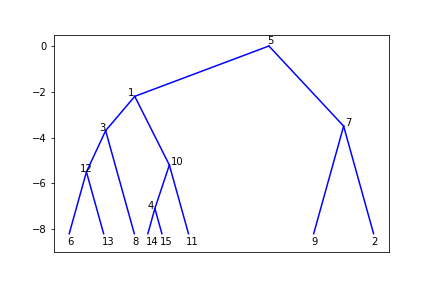
\includegraphics[width = 1.0\linewidth, trim={0 0 0 0}, clip=true]{figures/tree.png}
		\subcaption{Plot of mean fitness against allele frequency $p$}
		\label{fig:F}	
	\end{subfigure}
%	\hspace{0.1\linewidth}
%	\begin{subfigure}[t]{0.43\linewidth}
%		\centering
%		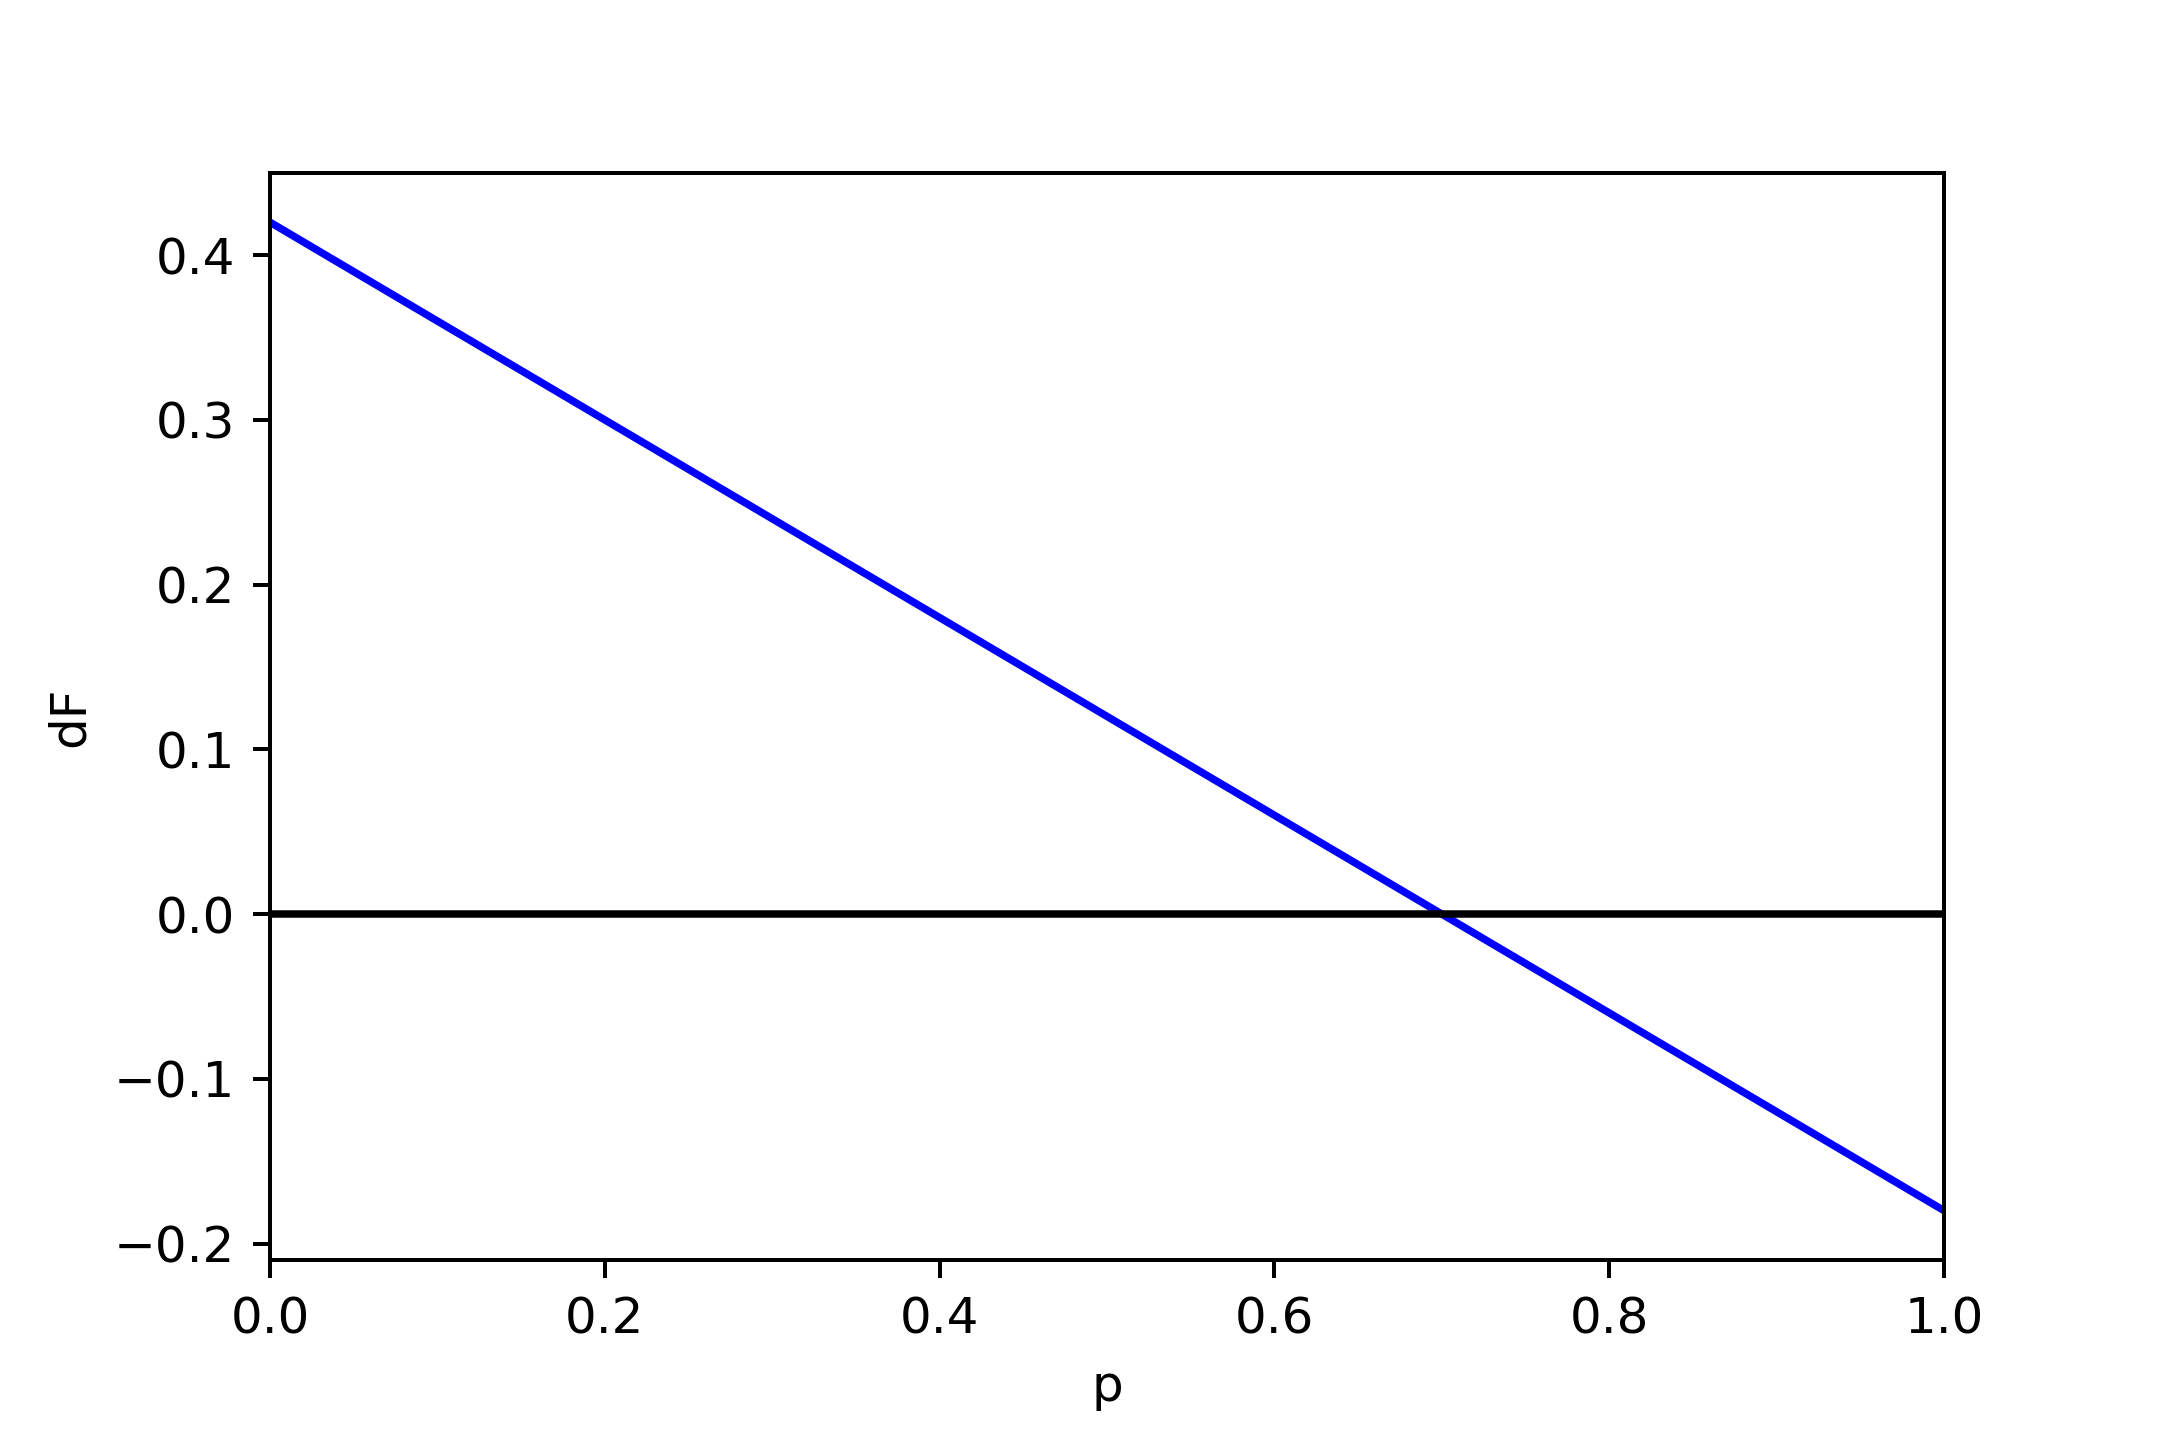
\includegraphics[width = 1.0\linewidth, trim={0 0 0 0}, clip=true]{dfitness.png}
%		\caption{$\dfrac{dF_{m}}{dp}$ against allele frequency $p$}
%		\label{fig:dF}
%	\end{subfigure}
\caption{}
\label{fig:tree}
\end{figure}


c)

given our topological sort function, we can now easily print out a relabelled tree where every daughter node has a lower number than its parent, simply by labelling each node according to it's position in the reverse of the topologically sorted list.


\begin{table}[h]
\centering
\begin{tabular}{ |c|c|c|c|c|c|}
\hline
 new label & original label & cumulative daughter nodes & internal nodes & leafnodes & distance from root \\
\hline
5 & 8 & 0 & 0 & 0 & 8.2 \\
8 & 14 & 0 & 0 & 0 & 8.2 \\
7 & 15 & 0 & 0 & 0 & 8.2 \\
4 & 2 & 0 & 0 & 0 & 8.2 \\
3 & 11 & 0 & 0 & 0 & 8.2 \\
2 & 6 & 0 & 0 & 0 & 8.2 \\
1 & 13 & 0 & 0 & 0 & 8.2 \\
\hline
6 & 12 & 2 & 2 & 0 & 5.5 \\
9 & 4 & 2 & 2 & 0 & 7.1 \\
10 & 7 & 2 & 2 & 0 & 3.5 \\
11 & 3 & 4 & 3 & 1 & 3.7 \\
12 & 10 & 4 & 3 & 1 & 5.2 \\
13 & 1 & 10 & 6 & 4 & 2.2 \\
14 & 5 & 14 & 8 & 6 & 0 \\
\hline
\end{tabular}
\caption{daughter nodes}
\label{tab:treesum}
\end{table}


we can also make this plot a relabelled graph

\begin{figure}[h]
	\centering
	\begin{subfigure}[t]{0.63\linewidth}
		\centering
		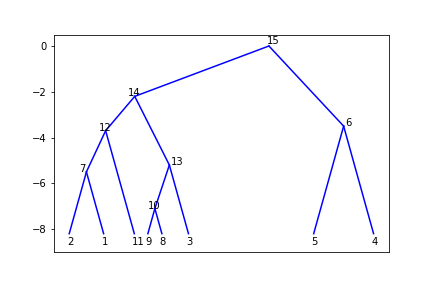
\includegraphics[width = 1.0\linewidth, trim={0 0 0 0}, clip=true]{figures/tree_relabelled.png}
		%\subcaption{Plot of mean fitness against allele frequency $p$}
		%\label{fig:F}	
	\end{subfigure}
%	\hspace{0.1\linewidth}
%	\begin{subfigure}[t]{0.43\linewidth}
%		\centering
%		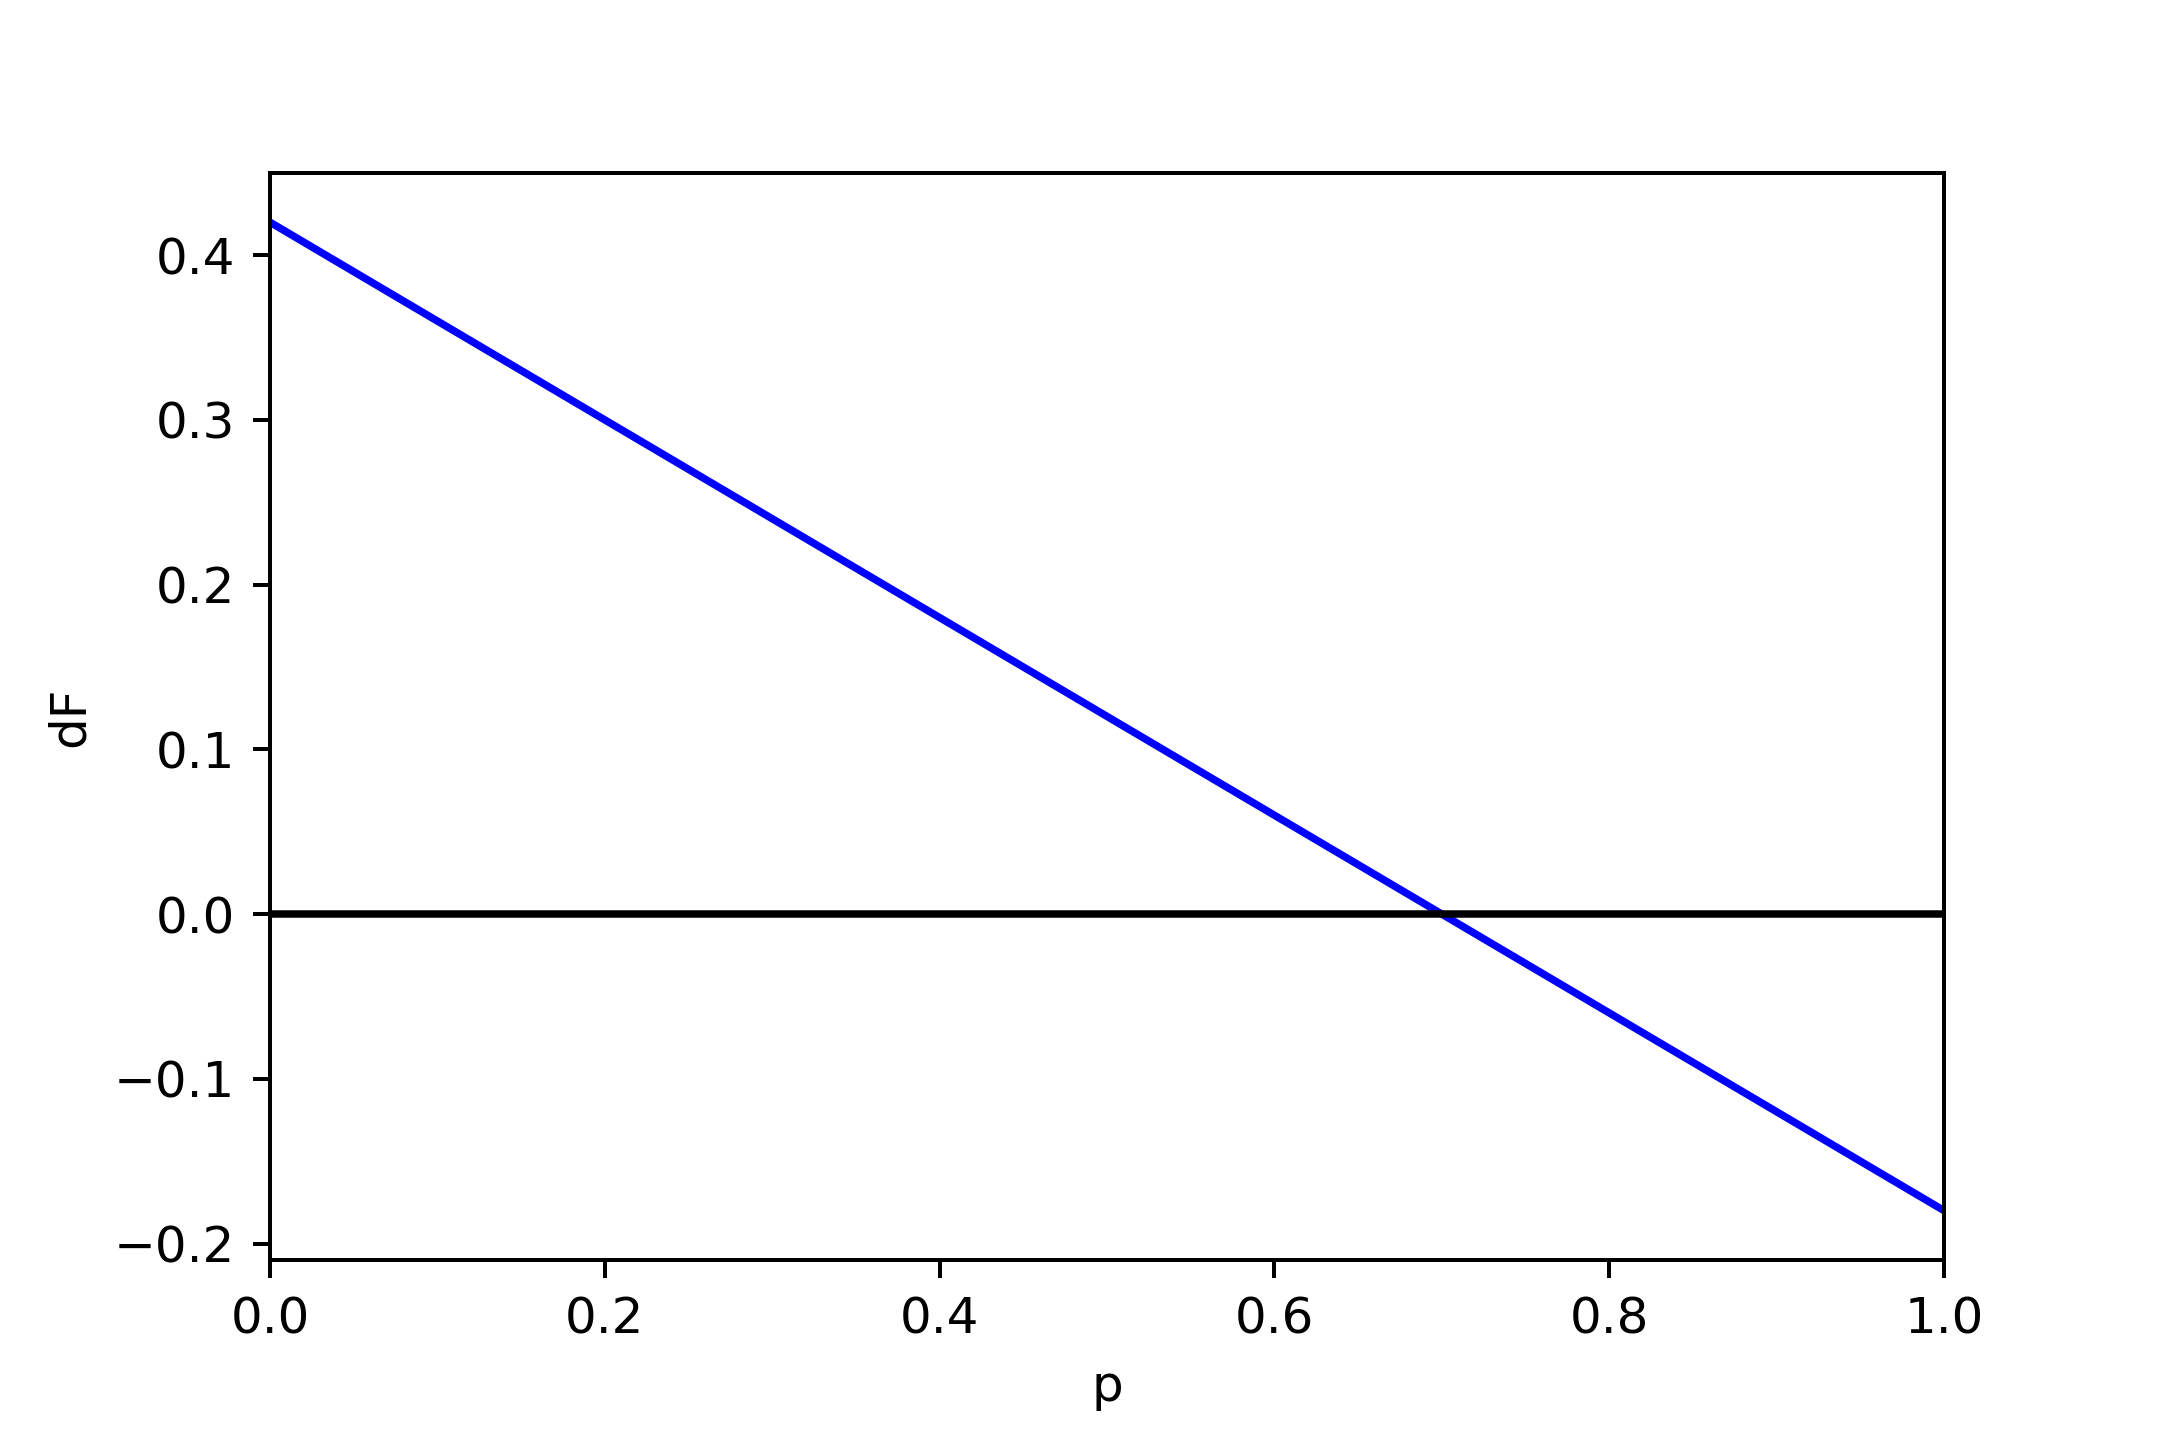
\includegraphics[width = 1.0\linewidth, trim={0 0 0 0}, clip=true]{dfitness.png}
%		\caption{$\dfrac{dF_{m}}{dp}$ against allele frequency $p$}
%		\label{fig:dF}
%	\end{subfigure}
\caption{relabelled tree}
\label{fig:tree_relab}
\end{figure}

\subsection{Time-dependent selection}

We consider an organisms with 1000 genes each of which can be fixed in state 0 or 1. We let $f_i^a$ denote the fitness advantage of gene $i$ in state $a$ and draw it from an exponential distribution with parameter 100.
At t=0, we assume state 1 to be beneficial and let $f_i^0 = -f_i^1$, $f_i^1 > 0$. We assume that no more than one gene is polymorphic at any time. Given a mutation in a gene, the probability of fixation is given by
\begin{equation}\label{eq:pfix}
p_{fix}(f_i^a) = \dfrac{1- e^{-2 f_i^a}}{1- e^{-2 N f_i^a}}
\end{equation}
Where N is the population size. We assume the lifespan of each polymorphism to be
\begin{equation}
\min{(10, \dfrac{2 \log{(N-1)}}{919 f_i^a})}
\end{equation}
We let N = 100 and use the natural logarithm.

We note that this particular system can be implemented in two different ways. In the first implementation, we consecutive mutations between the 0 and 1 states of a gene to be independent such that whenever a mutation occurs in a gene in state 1, we draw a new fitness $f_i^0 = -|f_i|$ and whenever a mutation occurs in state 0, we draw a new fitness $f_i^1 = +|f_i|$.

In the other implementations, the relative fitnesses of states 0 and 1 are fixed and we draw all $f_i^1$ at the beginning of the simulation corresponding to the system switching between two pre-defined alleles over the course of the simulation. On one hand, this justifies always having $f_i^0 < 0$ and $f_i^1 > 0$, but on the other hand it is unlikely that a second mutation in gene $i$ will exactly reverse the effect of the first mutation. In the following, we consider both of these interpretations.

The number of allele 1 over the 1000 loci for these two approaches have been plotted in figures \ref{fig:resample_trajec} and \ref{fig:constant_trajec}. We see that in both cases, an equilibrium state of $n_1 \approx 800$ has been reached after 500,000 timesteps.

\begin{equation}
n1 \cdot p(a=1 \rightarrow a=0) = n2 \cdot  p(a=0 \rightarrow a=1)
\end{equation}

This implies that the integral of the right side of the above figure must be equal to the integral of the left side. We can thus calculate the expected n1 analytically.

b)

We start sampling the $f$ values that lead to successful fixation after t=500,000 and run the simulation for an additional 2,500,000 timesteps. We then plot histograms showing the frequency of fixation for a given value of $f$ in figures \ref{fig:resample_hist} and \ref{fig:constant_hist}.

\begin{figure}[h]
	\centering
	\begin{subfigure}[t]{0.43\linewidth}
		\centering
		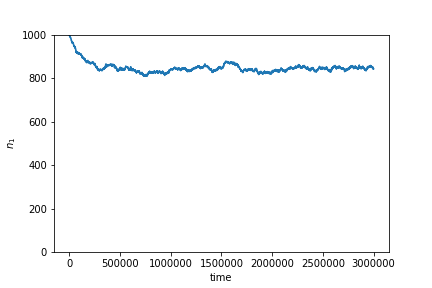
\includegraphics[width = 1.0\linewidth, trim={0 0 0 0}, clip=true]{figures/resample_selection_trajec.png}
		\subcaption{$n1$ as a function of simulated time}
		\label{fig:resample_trajec}	
	\end{subfigure}
	\hspace{0.1\linewidth}
	\begin{subfigure}[t]{0.43\linewidth}
		\centering
		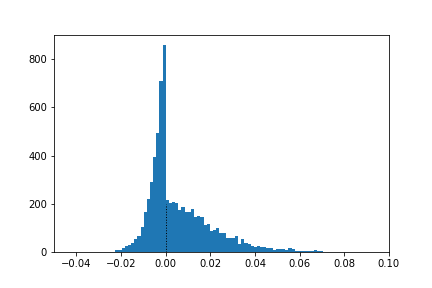
\includegraphics[width = 1.0\linewidth, trim={0 0 0 0}, clip=true]{figures/resample_selection_hist2.png}
		\caption{Frequency of fitnesses $f$ that fix in the population}
		\label{fig:resample_hist}
	\end{subfigure}
\caption{Simulation results when drawing a new $f_i$ whenever a mutation occurs.}
\label{fig:resample}
\end{figure}

We can explain the shape of the distribution of frequencies of fixation in the case of resampling by putting together three separate distributions (figure \ref{fig:alldists}). These are\\
1. the number of alleles in states 0 and 1 respectively since a 0 $\rightarrow$ 1 transition is associated with $f > 0$ and vice versa\\
2. The probability with which we draw a given f value if in state 0 for f>0 and in state 1 for f<1. This is given by the exponential distribution $e^{-\lambda|f|}$ with $\lambda = 100$.\\
3. the probability with which a mutation fixates given by equation \ref{eq:pfix}.
If we multiply these three probability distributions, we arrive at a theoretical distribution that resembles the simulated data very closely (figure \ref{fig:comb} suggesting that this is a good explanation for the observed data. The frequency distribution is thus given by
\begin{equation}\label{eq:dist1}
y \propto n_1 * exp(-|f|) * \dfrac{1- e^{-2 f}}{1- e^{-2 N f}}   f < 0
\end{equation}
\begin{equation}\label{eq:dist2}
y \propto n_0 * exp(-|f|) * \dfrac{1- e^{-2 f}}{1- e^{-2 N f}}   f > 0
\end{equation}

\begin{figure}[h]
	\centering
	\begin{subfigure}[t]{0.43\linewidth}
		\centering
		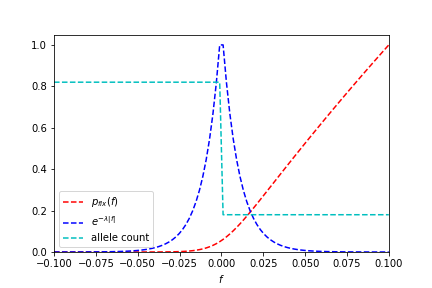
\includegraphics[width = 1.0\linewidth, trim={0 0 0 0}, clip=true]{figures/selection_dists.png}
		\subcaption{Distributions of alleles (cyan), frequency of drawing a given fitness (blue) and probability of fixation (red) as a function of fitness $f$.}
		\label{fig:alldists}	
	\end{subfigure}
	\hspace{0.1\linewidth}
	\begin{subfigure}[t]{0.43\linewidth}
		\centering
		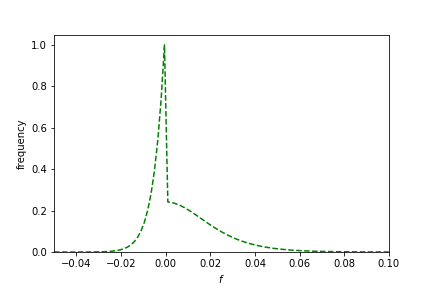
\includegraphics[width = 1.0\linewidth, trim={0 0 0 0}, clip=true]{figures/all_combined_dists.png}
		\caption{Product of the three distributions in (a). This distributions explains the observed form of the simulate data.}
		\label{fig:comb}
	\end{subfigure}
\caption{}
\label{fig:theory_resample}
\end{figure}

If instead we fix the values of $f$ at the beginning of the simulation, consecutibe mutations are no longer independent and we isntead observe a symmetric distribution of frequencies of fixation (figure \ref{fig:constant_hist}). Considering the set of all mutations in a single site $i$. Whenever it is in state 1, the probability of fixation is $p_1 = p_{fix}(f_0^i)$ and whenever it is in state 0 the probability of fixation is $p_0 = p_{fix}(f_1^i)$. This probability can be interpreted as a frequency of switching, and the average time between switching is thus the inverse of this frequency. However, because the state must switch back from 1 to 0 to switch from 0 to 1, in the limit of $t \rightarrow \infty$ where many switches occur, the average switching time for site i is given by the mean switching time from $0 \rightarrow 1$ and $1 \rightarrow 0$. Denoting this mean switching time $\tau_i$,

\begin{equation}
\tau_i \propto \dfrac{1}{2p_1} + \dfrac{1}{2p_0} = \dfrac{1- e^{-2 N f_i^0}}{2- 2e^{-2 f_i^0}} + \dfrac{2- 2e^{-2 N f_i^1}}{1- e^{-2 f_i^1}}
\end{equation}
The average frequency of switching for site i is thus $\omega \propto \dfrac{1}{\tau_i}$.
Since the distribution of fitnesses is given by $e^{-\lambda |f_i|}$, the probability distribution of fixation as a function of $f$ is therefore given by $\dfrac{1}{\tau_i} e^{-\lambda |f_i|} $.
This has been plotted in figure \ref{fig:simconst} and we see that it fits very well with the simulated data.

\begin{figure}[h]
	\centering
	\begin{subfigure}[t]{0.32\linewidth}
		\centering
		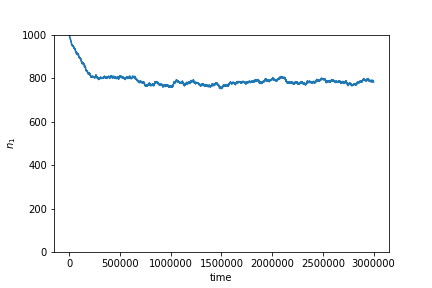
\includegraphics[width = 1.0\linewidth, trim={0 0 0 0}, clip=true]{figures/constant_selection_trajec.png}
		\subcaption{$n1$ as a function of simulated time}
		\label{fig:constant_trajec}	
	\end{subfigure}
	\hspace{0.01\linewidth}
	\begin{subfigure}[t]{0.32\linewidth}
		\centering
		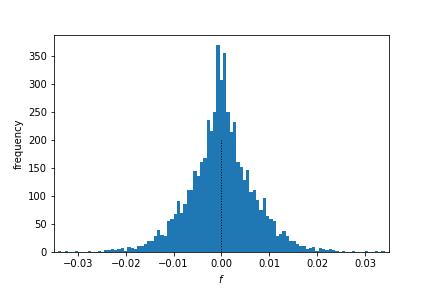
\includegraphics[width = 1.0\linewidth, trim={0 0 0 0}, clip=true]{figures/constant_selection_hist2.png}
		\caption{Frequency of fitnesses $f$ that fix in the population}
		\label{fig:constant_hist}
	\end{subfigure}
	\begin{subfigure}[t]{0.32\linewidth}
		\centering
		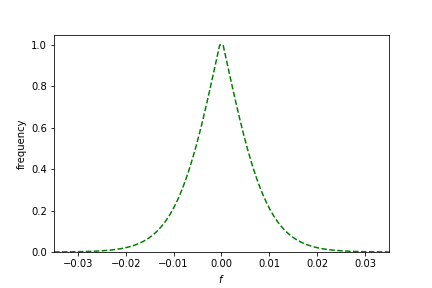
\includegraphics[width = 1.0\linewidth, trim={0 0 0 0}, clip=true]{figures/sym_combined_dists.png}
		\subcaption{Predicted frequencies of fixation given by $\dfrac{e^{-\lambda |f_i|}}{\tau_i} $}.
		\label{fig:simconst}	
	\end{subfigure}
\caption{Simulation results when drawing a new $f_i$ whenever a mutation occurs.}
\label{fig:tree}
\end{figure}


c)

We now let the environment change at a frequency determined by a poisson distribution with rate $\tau = 5*10^(-6)$. Upon a change in environment, fitnesses of alleles 1 and 0 reverse such that $f_i^1 < 0$ and $f_i^0 > 0$ for all i. We see in figures \ref{fig:changing_resample_trajec} and \ref{fig:changing_constant_trajec} that this leads to oscillations in $n_1$ as allele 1 becomes alternatingly more and less fit compared to allele 0 at each site.

In the limit of $t \rightarrow \infty$ this averages the populations of state 1 and state 2 which in turn leads to the resampling and fixed fitness strategies being equivalent since consecutive fixations can now occur with the same change in fitness $\Delta f$ for a single site i in the fixed fitness model. This is evident from figures \ref{fig:changing_resample} and \ref{fig:changing_constant}.
However, we do note that we still sample fitness space less thoroughly with fixed fitnesses.

\begin{figure}[h]
	\centering
	\begin{subfigure}[t]{0.32\linewidth}
		\centering
		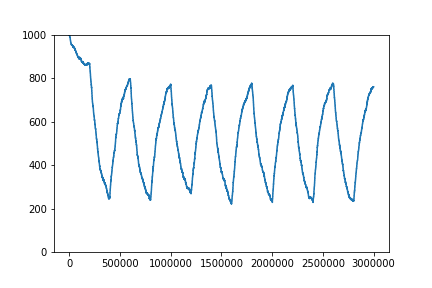
\includegraphics[width = 1.0\linewidth, trim={0 0 0 0}, clip=true]{figures/changing_resample_selection_trajec.png}
		\subcaption{$n1$ as a function of simulated time}
		\label{fig:changing_resample_trajec}	
	\end{subfigure}
	\hspace{0.01\linewidth}
	\begin{subfigure}[t]{0.32\linewidth}
		\centering
		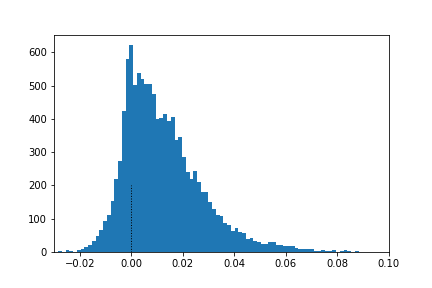
\includegraphics[width = 1.0\linewidth, trim={0 0 0 0}, clip=true]{figures/changing_resample_selection_hist2.png}
		\caption{Frequency of fitnesses $f$ that fix in the population}
		\label{fig:changing_resample_hist}
	\end{subfigure}
	\begin{subfigure}[t]{0.32\linewidth}
		\centering
		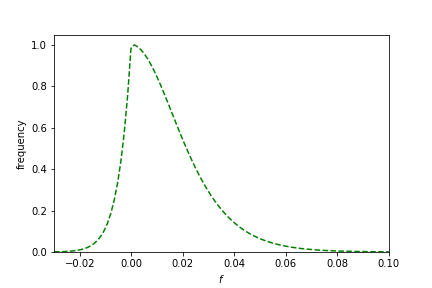
\includegraphics[width = 1.0\linewidth, trim={0 0 0 0}, clip=true]{figures/no_n_combined_dists.png}
		\caption{Predicted frequencies of fixation given by $e^{-\lambda |f|} p_{fix}(f)$}
		\label{fig:changing_resample_predict}
	\end{subfigure}
\caption{Simulated and predicted behavior of system with resampling and changing environment}
\label{fig:changing_resample}
\end{figure}

\begin{figure}[h]
	\centering
	\begin{subfigure}[t]{0.32\linewidth}
		\centering
		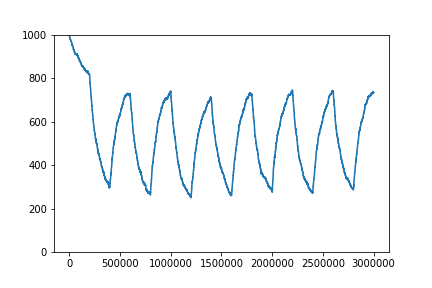
\includegraphics[width = 1.0\linewidth, trim={0 0 0 0}, clip=true]{figures/changing_selection_trajec.png}
		\subcaption{$n1$ as a function of simulated time}
		\label{fig:changing_constant_trajec}	
	\end{subfigure}
	\hspace{0.01\linewidth}
	\begin{subfigure}[t]{0.32\linewidth}
		\centering
		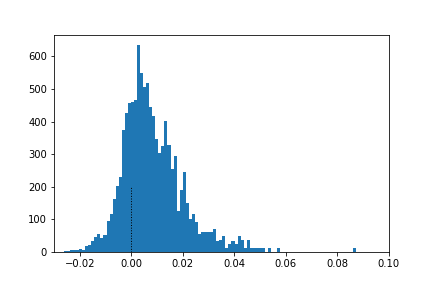
\includegraphics[width = 1.0\linewidth, trim={0 0 0 0}, clip=true]{figures/changing_selection_hist2.png}
		\caption{Frequency of fitnesses $f$ that fix in the population}
		\label{fig:changing_constant_hist}
	\end{subfigure}
	\begin{subfigure}[t]{0.32\linewidth}
		\centering
		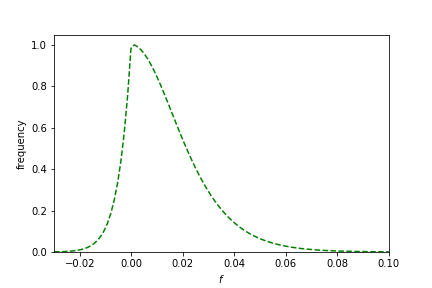
\includegraphics[width = 1.0\linewidth, trim={0 0 0 0}, clip=true]{figures/no_n_combined_dists.png}
		\caption{Predicted frequencies of fixation given by $e^{-\lambda |f|} p_{fix}(f)$}
		\label{fig:changing_constant_predict}
	\end{subfigure}
\caption{Simulated and predicted behavior of system with constant $|f_i|$ and changing environment}
\label{fig:changing_constant}
\end{figure}

In the long time limit of a changing environment, $\braket{n_1} = \braket{n_2}$ where $\braket{}$ denotes a time average. The frequency distribution is thus given by equations \ref{eq:dist1} and \ref{eq:dist2} with $n_1 = n_2$, giving
\begin{equation}\label{eq:shift_non}
y \propto exp(-|f|) * \dfrac{1- e^{-2 f}}{1- e^{-2 N f}}
\end{equation}
This has been plotted in figures \ref{fig:changing_constant_predict} and \ref{fig:changing_resample_predict} and we see that it fits well with the data in both cases.

d)
As $\tau$ becomes large, the frequency of changes in the environment become increasingly frequent, making the time average approximation increasingly accurate. This leads to the distribution of fitnesses that fix becoming increasingly similar to equation \ref{eq:shift_non}. Similar results are obtained with resampling. In the present case of constant fitnesses, a better fit to the predicted frequencies would be obtained with an increased number of genes.

\begin{figure}[h]
	\centering
	\begin{subfigure}[t]{0.24\linewidth}
		\centering
		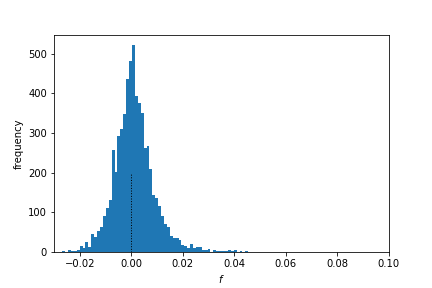
\includegraphics[width = 1.0\linewidth, trim={0 0 0 0}, clip=true]{figures/tau5e7_selection_hist2.png}
		\subcaption{$\tau = 10^{-7}$}
		\label{fig:t7}	
	\end{subfigure}
	\hspace{0.01\linewidth}
	\begin{subfigure}[t]{0.24\linewidth}
		\centering
		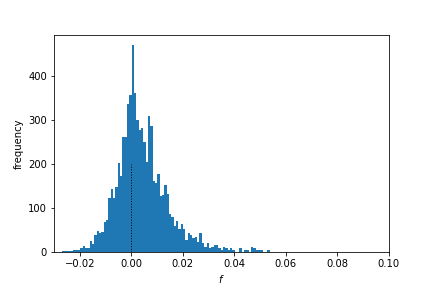
\includegraphics[width = 1.0\linewidth, trim={0 0 0 0}, clip=true]{figures/tau5e5_selection_hist2.png}
		\caption{$\tau = 10^{-6.5}$}
		\label{fig:t65}
	\end{subfigure}
	\begin{subfigure}[t]{0.24\linewidth}
		\centering
		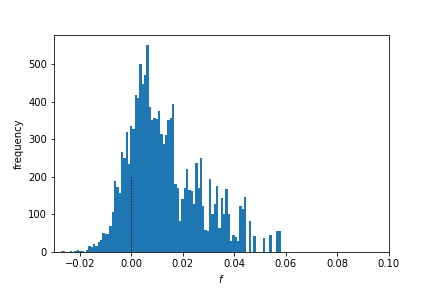
\includegraphics[width = 1.0\linewidth, trim={0 0 0 0}, clip=true]{figures/tau5e3_selection_hist2.png}
		\caption{$\tau = 10^{-4}$}
		\label{fig:t4}
	\end{subfigure}
	\begin{subfigure}[t]{0.24\linewidth}
		\centering
		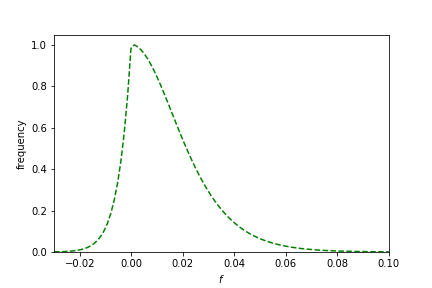
\includegraphics[width = 1.0\linewidth, trim={0 0 0 0}, clip=true]{figures/no_n_combined_dists.png}
		\caption{Predicted}
		\label{fig:pred}
	\end{subfigure}
\caption{Frequency of fitnesses $f$ that fix in the population for a changing environment with fixed fitnesses $|f|$. As $\tau$ increases, this increasingly resembles the predicted distribution resulting from a time average of the populations $n_1$ and $n_0$.}
\label{fig:changing_constant}
\end{figure}

This can also be rationalized by looking at the $n_1$ curves where for small $\tau$ we only see a single or a few transitions, whereas for large $\tau$ transitions occur very rapidly and the equilibrium state has $n_1 \approx n_2 \approx 500$.

\begin{figure}[h]
	\centering
	\begin{subfigure}[t]{0.24\linewidth}
		\centering
		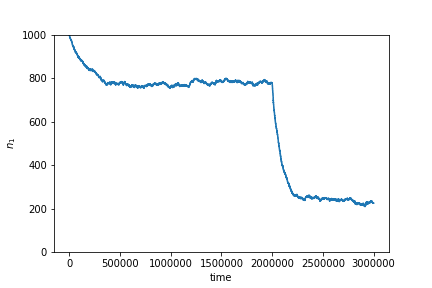
\includegraphics[width = 1.0\linewidth, trim={0 0 0 0}, clip=true]{figures/tau5e7_selection_trajec.png}
		\subcaption{$\tau = 10^{-7}$}
		\label{fig:t7}	
	\end{subfigure}
	\hspace{0.01\linewidth}
	\begin{subfigure}[t]{0.24\linewidth}
		\centering
		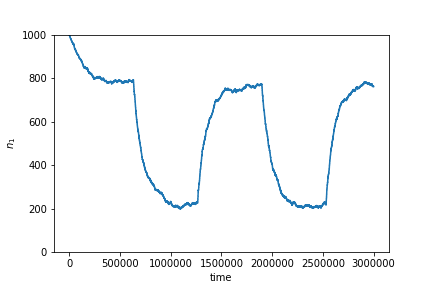
\includegraphics[width = 1.0\linewidth, trim={0 0 0 0}, clip=true]{figures/tau5e5_selection_trajec.png}
		\caption{$\tau = 10^{-6.5}$}
		\label{fig:t65}
	\end{subfigure}
	\begin{subfigure}[t]{0.24\linewidth}
		\centering
		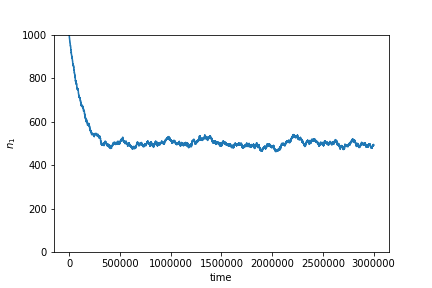
\includegraphics[width = 1.0\linewidth, trim={0 0 0 0}, clip=true]{figures/tau5e3_selection_trajec.png}
		\caption{$\tau = 10^{-4}$}
		\label{fig:t4}
	\end{subfigure}

\caption{$n1$ as a function of simulated time for a changing environment with fixed fitnesses $|f|$. As $\tau$ increases, oscillations become increasingly fast, allowing us to take a time average of the populations $n_1$ and $n_0$.}
\label{fig:changing_constant_trajecs}
\end{figure}

We thus see that as $\tau$ increases, the proportion of fixed mutations that are beneficial (i.e. has $f > 0$) increases until it reaches the limiting distribution given by equation \ref{eq:shift_non}.

e)
\textit{Drosophila} have a relatively short generation time of $\approx$2 weeks. Changes in the environment due to factors such as changing seasons thus occurs over a timescale that allows for fixation of mutations in small populations within a single season. This scenario is qualitatively similar to the scenario considered above, where e.g. alleles that are more beneficial during the summer can arise and fix during the warmer months while alleles that are more beneficial in the winter can arise and fix during the colder months. As is evident form figure \ref{fig:t65}, this will lead to the population having a large proportion of beneficial mutations if the relative timescales of the generation time and change in environment is appropriate.

As is evident from figure \ref{fig:changing_constant_trajecs}, this can lead to there being a number of beneficial mutations at any one time, but at a later time these may turn out to be detrimental and thus be cleared from the population. This does not lead to the mean fitness of the population increasing over long timescales, but it does lead to the population being fitter at a given time of year, albeit there will be a delay corresponding to the fixation time of the mutation.

This particular scenario is likely to be more similar to the model with resampling of fitnesses rather than fixed fitnesses since we can imagine there to be a set of mutations $\{1_j\}$ that are more beneficial during the summer and a set of mutations $\{0_j\}$ that are more beneficial during the winter, and while the population can change between these two states, it is unlikely that mutations are exactly reversed. Instead, the population will likely sample genotype space in a more continous manner where mutations in a given gene can have different fitness advantages depending on how it affects the resulting protein and its expression level.


\subsection{Ancestral inference}

\subsection{Neanderthal introgression}



\newpage

\section*{Appendix}

\lstinputlisting[language=python]{trees.py}

\end{document}